\documentclass[a4,12pt]{report}

\usepackage[french]{babel}
\usepackage[utf8]{inputenc}
\usepackage[T1]{fontenc}
\usepackage{graphicx}

% Title Page
\title{ Rapport - TP IMA208}
\author{Renata PORCIUNCULA BAPTISTA}


\begin{document}
\maketitle

\chapter*{Introduction}
L'objective de ce rapport est présenter des résultats et conclusions des implémentations d'algorithme de traitement géometrique 3D. Les méthodes visent sont HPSS et APSS.
\section*{Partie I - HPSS}
\subsection*{1- L'ensemble aléatoire}

Nous avons utilisé $N=20000$, où $N$ est le numéro de points. Les images \ref{fig:1}, \ref{fig:2}, \ref{fig:3} montrent les résultats pour le méthode HPSS.
\begin{figure}[!h]
	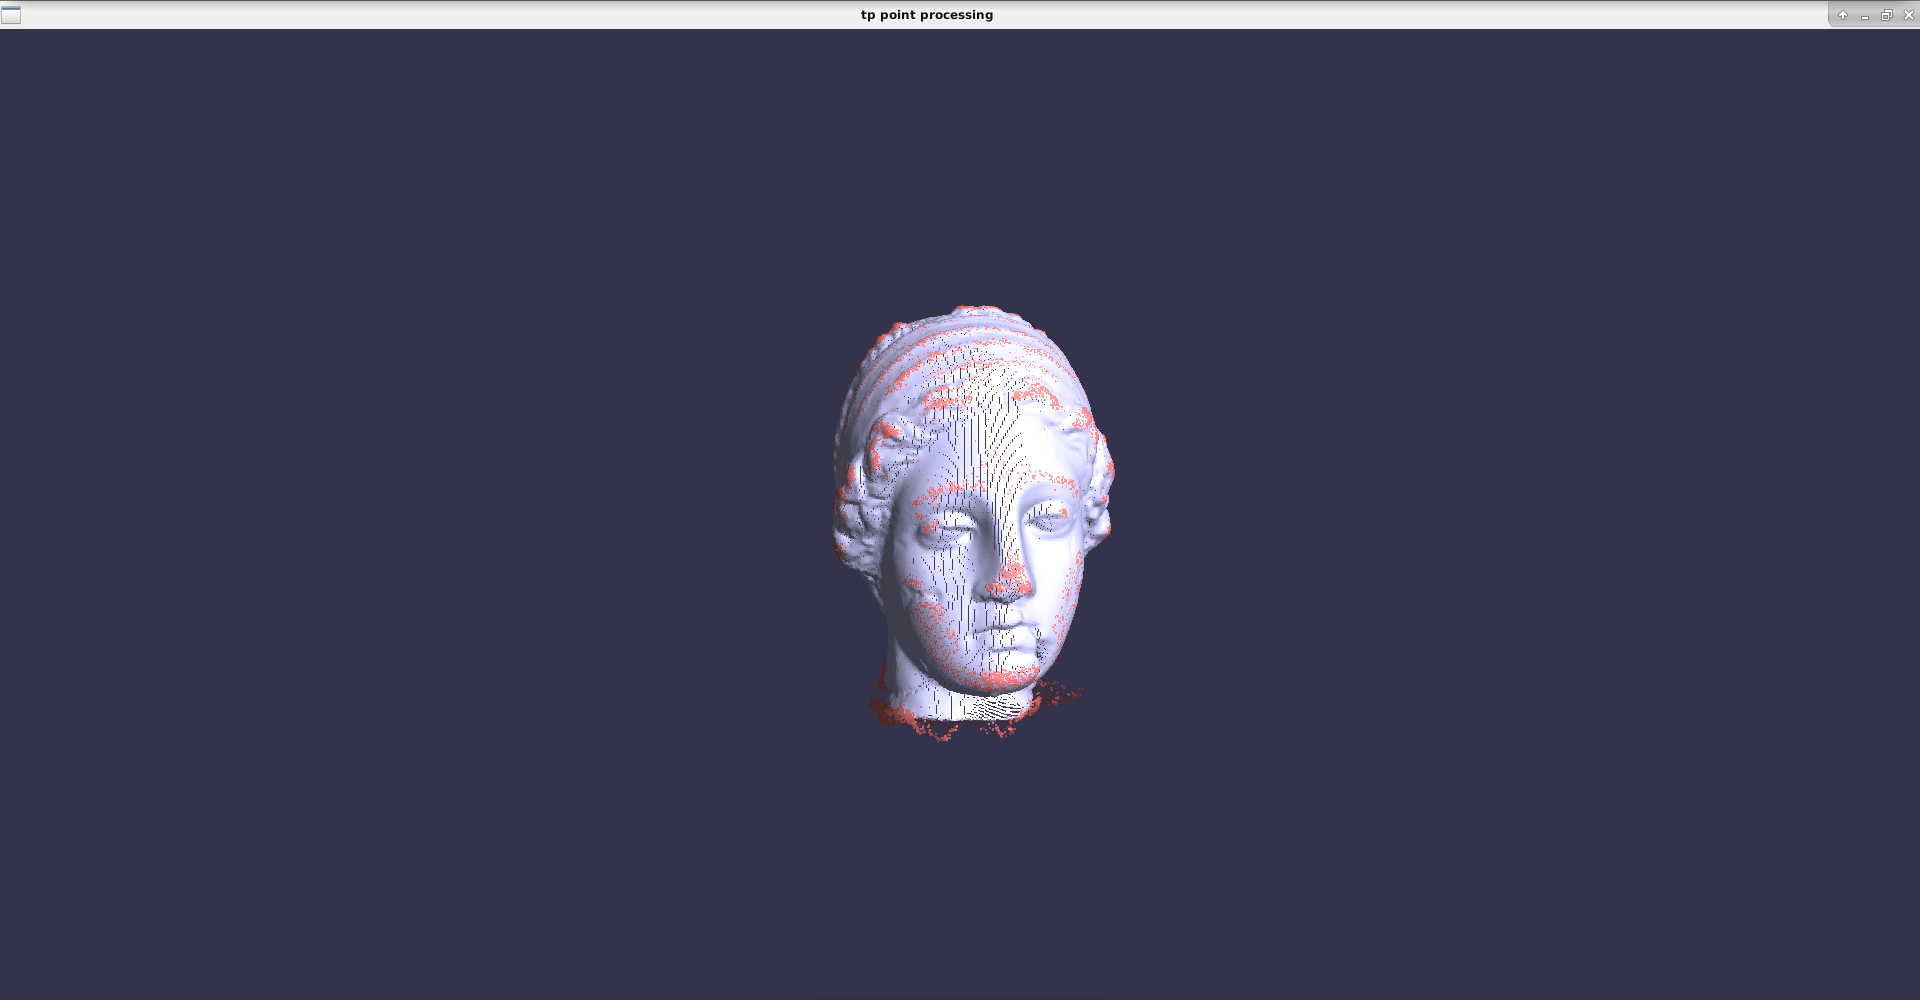
\includegraphics[width=\linewidth]{figs/primeiro_casp.png}
	\caption{Résultat HPSS - front}
	\label{fig:1}
\end{figure}
\begin{figure}[!h]
	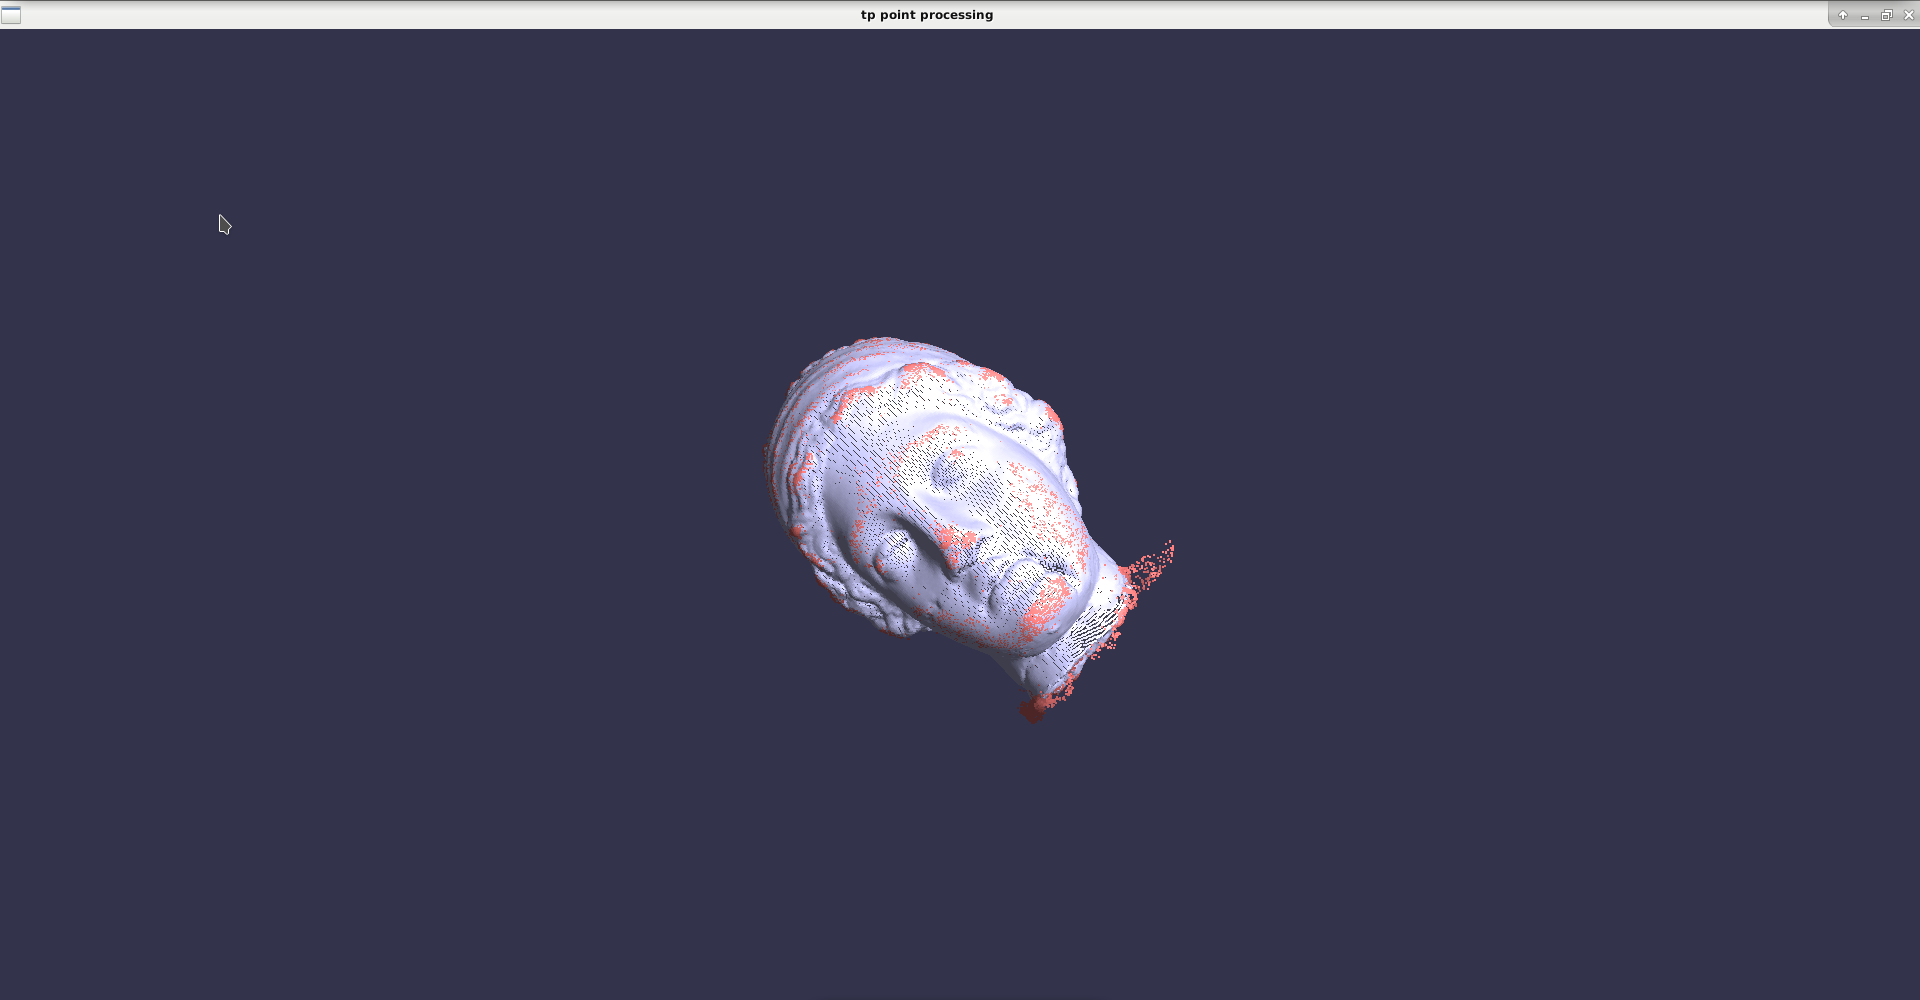
\includegraphics[width=\linewidth]{figs/primeiro_caso_diag.png}
	\caption{Résultat HPSS - diag}
	\label{fig:2}
\end{figure}
\begin{figure}[!h]
	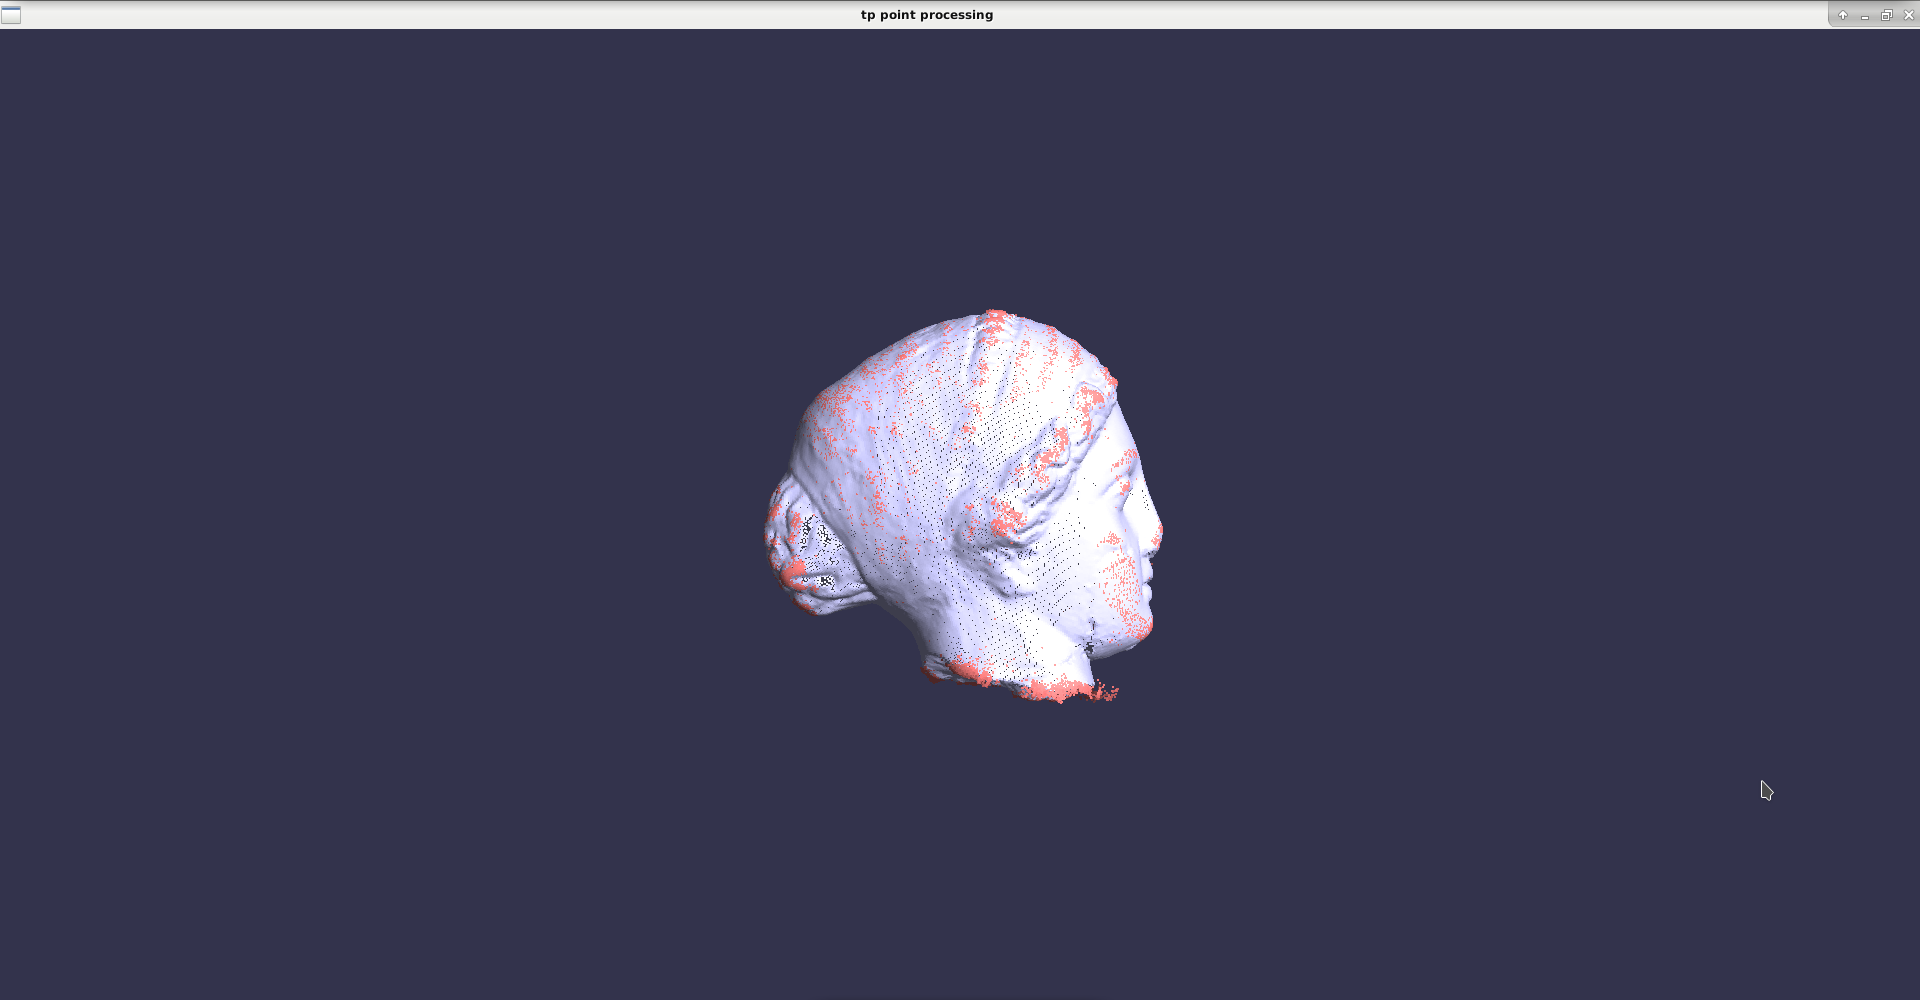
\includegraphics[width=\linewidth]{figs/primeiro_caso_lat.png}
	\caption{Résultat HPSS - lat}
	\label{fig:3}
\end{figure}


\subsection*{2- Noyau gaussien}

Nous avons utilisé $N=20000$, où $N$ est le numéro de points. Les images \ref{fig:4}, \ref{fig:5} montrent les résultats pour le méthode HPSS avec différents moyennes et écart type.

\begin{figure}[!h]
	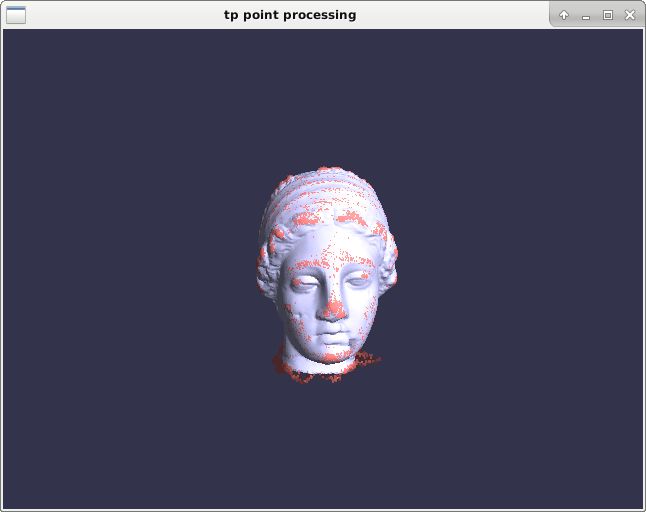
\includegraphics[width=\linewidth]{figs/gaussian_sem_bruit_0_1.png}
	\caption{Résultat HPSS - radius 0.2}
	\label{fig:4}
\end{figure}
\begin{figure}[!h]
	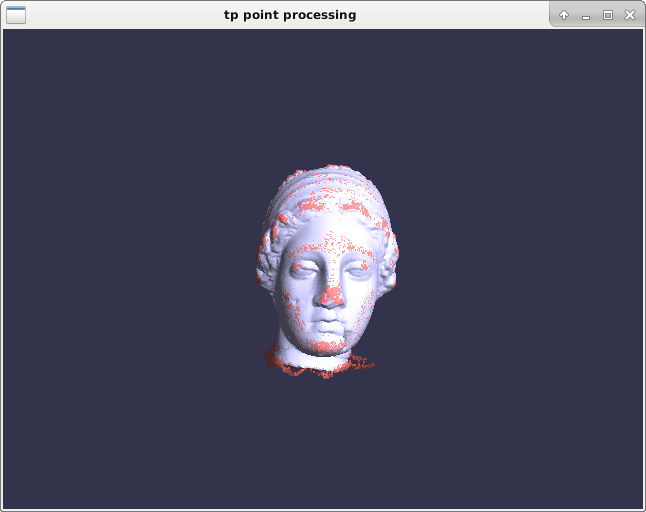
\includegraphics[width=\linewidth]{figs/gaussian_sem_bruit_0_5.png}
	\caption{Résultat HPSS - radius 0.4}
	\label{fig:5}
\end{figure}

Le plus grand le rayon de filtrage, plus de points sont utilisés pour définir la projection. Plus robuste.
Le plus plut petit le rayon de filtrage, moins de points utilisés pour définir la projection. 


\subsection*{3- Noyau gaussien avec le bruit}


\section*{Part II - APSS}
\subsection*{1- APSS versus HPSS} 
Nous n'avons pas reussi à coder l'APSS.

%\begin{abstract}
%\end{abstract}

\end{document}          
